\documentclass[11.5pt]{sig-alternate} % sets document style to sig-alternate
% packages
% typesetting
%\usepackage{dirtytalk} % typset quotations easier (\say{stuff})
\usepackage{hanging} % hanging paragraphs
\usepackage[defaultlines=3,all]{nowidow} % avoid widows
\usepackage[pdfpagelabels=false]{hyperref} % produce hypertext links, includes backref and nameref
\usepackage{xurl} % defines url linebreaks, loads url package
\usepackage{microtype}
%\usepackage[super]{nth} % easily create superscript ordinal numbers with \nth{x}
\usepackage{textcomp}
\newcommand{\texttildemid}{\raisebox{0.4ex}{\texttildelow}}
% layout
%\usepackage{enumitem} % control layout of itemize, enumerate, description
\usepackage{fancyhdr} % control page headers and footers
\usepackage{float} % improved interface for floating objects
%\usepackage{multicol} % intermix single and multiple column pages
% language
\usepackage[utf8]{inputenc} % accept different input encodings
\usepackage[english]{babel} % multilanguage support
% misc
\usepackage{graphicx} % builds upon graphics package, \includegraphics
%\usepackage{lastpage} % reference number of pages
%\usepackage{comment} % exclude portions of text (?)
\usepackage{xcolor} % color extensions
\usepackage[backend=biber, style=apa]{biblatex} % sophisticated bibliographies % necessary for HTML to display author info and date on abstract page
\usepackage{csquotes} % advanced quotations, makes biblatex happy
\usepackage{authblk} % support for footnote style author/affiliation
% tables and figures
\usepackage{tabularray}
%\usepackage{array} % extend array and tabular environments
\usepackage{caption} % customize captions in figures and tables (rotating captions, sideways captions, etc)
%\usepackage{cuted} % allow mixing of \onecolumn and \twocolumn on same page
\usepackage{multirow} % create tabular cells spanning multiple rows
%\usepackage{subfigure} % deprecated, support for manipulation of small figures
%\usepackage{tabularx} % extension of tabular with column designator "x", creates paragraph-like column whose width automatically expands
%\usepackage{wrapfig} % allows figures or tables to have text wrapped around them
%\usepackage{booktabs} % better rules
% dummy text
%\usepackage{blindtext} % blind text dummy text
%\usepackage{kantlipsum} % Kant style dummy text
\usepackage{lipsum} %lorem ipsum dummy text
% other helpful packages may be booktabs, longtable, longtabu, microtype

\pagestyle{fancy} % sets pagestyle to fancy for fancy headers and footers

% header and footer
% modern way to set header image
\renewcommand{\headrulewidth}{0pt} % defines thickness of line under header
\renewcommand{\footrulewidth}{0pt} % defines thickness of line above header
\setlength\headheight{80.0pt} % sets height between top margin and header image, effectively moves page contents down
\addtolength{\textheight}{-80.0pt} % seems to affect the lower height. maybe only works properly if footer numbers enabled?
\fancyhf{}
\fancyhead[CE, CO]{
\includegraphics[width=\textwidth]{headerImage.png}}
% footer
%\fancyfoot[LE,LO]{Article Title Here \\ DOI: }% left footer article title and doi
%\fancyfoot[CE,CO]{{}} % center footer empty
%\fancyfoot[RE,RO]{\thepage} % right footer page numbers
%\pagenumbering{arabic} % arabic (1, 2, 3) numbering in footer

\hypersetup{colorlinks=true,urlcolor=blue} % sets link color to blue
\urlstyle{same} % sets url typeface to same as rest of text

% set caption and figure to italics, label bold, left align captions, does not transfer to HTML
\captionsetup{labelfont=bf, font={large, it}, justification=raggedright, singlelinecheck=false}
\renewcommand\theContinuedFloat{\alph{ContinuedFloat}}

%this next bit is confusing, but essentially changes the width of the abstract. Seems to have been copied from this https://tex.stackexchange.com/questions/151583/how-to-adjust-the-width-of-abstract
\let\oldabstract\abstract
\let\oldendabstract\endabstract
\makeatletter %changes @ catcode to enable modification (in parsep)
\renewenvironment{abstract} %alters the abstract environment
{\renewenvironment{quotation}%
               {\list{}{\addtolength{\leftmargin}{1em} % change this value to add or remove length to the the default ?
                        \listparindent 1.5em%
                        \itemindent    \listparindent%
                        \rightmargin   \leftmargin%
                        \parsep        \z@ \@plus\p@}%
                \item\relax}%
               {\endlist}%
\oldabstract}
{\oldendabstract}
\makeatother %changes @ catcode to disable modification

% checks
% italics -
% links -
% dashes
% tildes
\begin{document}

\title{Tools Enabling a Student Who Is Blind in a Liberal Arts
Chemistry Laboratory Course}

\author[1]{\large \color{blue}Jessica Michael}
\author[2]{\large \color{blue}H. David Wohlers*}
\affil[1]{Parkway North Schools, St. Louis, MO}
\affil[2]{Truman State University}
\toappear{}
%% ABSTRACT
\maketitle
\begin{@twocolumnfalse} 
\begin{abstract}
\item 
\textit {Chemistry laboratories ordinarily involve a number of visual observations and require qualitative and quantitative explanations of these observations. A student with blindness at Truman State University successfully completed the laboratory portion of the nonmajors liberal arts chemistry course with the assistance of a senior undergraduate chemistry education major, the guidance of a chemistry professor with blindness, and a variety of alternative laboratory methods. Volumes were measured using a notched syringe or the graduated cylinder pipet technique. Changes in color were measured by a Color Analysis Laboratory Sensor (CALS) and a Submersible Audio Light Sensor (SALS). Balance and Vernier probe measurements were recorded using Vernier data acquisition software (Logger Pro 3.6) and Job Access with Speech (JAWS) screen review software. This paper reports the impact of these alternative methods on the level of participation of the student with blindness for the following experiments: Density Determination, Flame Emissions Tests, Simulation of the Measurement of Hemoglobin in the Blood Using Spectrophotometry, the Investigation of Hydrates, the Study of Chemical Reactions in Everyday Life, and Titrations. The Solutions, the Soap-Making, and Paper Chromatography laboratories are not reported. All the laboratories except the Density laboratory are part of the Chemistry 100 curriculum at Truman State University (“CHEM 100”, 2010).}
\\ \\
Keywords: chemistry, laboratory, blind/low vision, accessibility
\end{abstract}
\end{@twocolumnfalse}

%% AUTHOR INFORMATION

\textbf{*Corresponding Author, H. David Wohlers}\\
\href{mailto: (wohlers@truman.edu) }{(wohlers@truman.edu)} \\
\textit{Submitted January 23rd, 2019 }\\
\textit{Accepted February 12th, 2019} \\
\textit{Published online March 28th, 2019 } \\
\textit{DOI:10.14448/jsesd.11.0010} \\
\pagebreak
\clearpage

\begin{large}
\section*{A STUDENT WITH BLINDNESS IN A LIBERAL ARTS CHEMISTRY LABORATORY \\COURSE}

According to the College Freshmen with Disabilities: A Biennial Statistical Profile, approximately 10.4\% of workers are people with disabilities with only 2.7\% involved in the science and engineering disciplines (American Council on Education, 1999). This small percentage is not a result of a lack of interest in science but a lack of access to science (Wexler, 1961). To prevent discrimination against individuals with disabilities and to uphold their equal participation in society, Congress established a legal framework of the full range of educational opportunities for persons with disabilities. These laws include the Rehabilitation Act of 1973; the Individuals with Disabilities Education Act (IDEA) of 1975; the Americans with Disabilities Act (ADA) of 1990; the 1997 Amendments to IDEA; and the Amendments to IDEA 2004. Educators have a defined set of responsibilities to ensure that no qualified students with disabilities can be excluded or deprived of benefits based on their disabilities according to Section 504 of the Rehabilitation Act of 1973. Most students who were blind and low-vision (BLV) did not participate in laboratory activities or they were severely limited before the inclusion laws were effective. With newly developed adaptive tools and other accommodations, students with disabilities can be fully included in the classroom because “a physical disability should never exclude a student from an educational activity as important as laboratory work” (Miner, Nieman, Swanson, \& Woods, 2001). All students should obtain a basic understanding of chemistry and science to become well-educated citizens, capable of making decisions and participating in day-to-day life (Wexler, 1961).

The paucity of published articles pertaining to laboratory accommodations for students who are blind or with low-vision are reviewed by Wexler (1961), Cetera (1983), and Supalo et al (2007). Some case studies describe methods and adaptations that involve students with BLV in the science classroom via new or adapted curricula. These cases, however, have not been duplicated to test their reliability, and they do not include post-secondary scenarios (Erwin, Perkins, Ayala, Fine, \& Rubin, 2001; Supalo et al, 2009; Wild \& Allen, 2009). By using computers with Vernier software along with three-dimensional manipulatives, more students with disabilities can participate in chemistry classrooms and laboratories, giving them a more “hands-on” experience (Supalo et al, 2007). These tools and accompanying audio descriptions enable students to acquire and retain scientific information (Schmeidler \& Kirchner, 2007). The expanding resources available on the internet give teachers ideas for making and acquiring three-dimensional manipulatives. Generally, these websites and online journal entries are lists of tools and their uses (Mallouk et al, 2010; Supalo, 2005; Supalo, Mallouk, Rankel, Amorosi, \& Graybill, 2008; Supalo et al, 2009; Rankel \& Winograd, 2010). It is essential to continue developing these ideas and investigating their efficacies to attain an inclusive environment for both the lecture and laboratory components of the class. 
 
A student with blindness at Truman State University successfully completed the laboratory portion of the nonmajors liberal arts chemistry course with the assistance of a senior undergraduate chemistry education major and the guidance of a chemistry professor with blindness. Few articles pertaining to college students with BLV succeeding in introductory chemistry courses have been published despite an occasional paper or poster presented at meetings of the American Chemical Society Division of Chemical Education, The National Science Teachers Association, or the American Association for the Advancement of Science. This case study provides a description of the techniques used and their effectiveness in specific laboratory activities. Not all the laboratory experiments performed during the semester as part of the Chemistry 100 laboratory curriculum are included in this case study; the solutions, the soap-making and paper chromatography laboratories are not reported. The student with blindness did not successfully complete every activity independently. Ideas and tips for implementing those that worked well are incorporated. 

\subsection*{A Case Study}

The nonmajors chemistry course serves as a basic introduction to the principles of modern chemistry and their applications to social, economic, and political issues (“CHEM 100”, 2010). An English education student with blindness enrolled in this course to fulfill a science liberal arts requirement. She voluntarily contributed to this project to help future students who are blind or low-vision succeed in chemistry courses (Wohlers \& Hoffmann, 2008). This class and laboratory were her first experiences with science since early high school. 

The laboratory portion of this course posed many obstacles due to the required techniques, visual observations, and visual confirmations (“CHEM 100”, 2010). To meet the laboratory requirements of the course and to enhance the learning experience the student, the assistant, and the chemistry professor with blindness met once per week for approximately three hours in his  faculty research laboratory. 

The student began the course with trepidation because she was uncomfortable around fire and fragile objects. She also admitted to having difficulty with her spatial awareness and abilities to navigate. She often joked about expecting to “blow up the school,” but her continual positive attitude and unending determination allowed her to succeed in the course. To prevent frustration and encourage her positive attitude, the team adopted the suggestion of Willoughby and Duffy (1989) and Supalo et al (2009) to require her to read the laboratory handout and instructions prior to entering the laboratory.

The assistant helped the student learn to safely yet independently manipulate various pieces of equipment, move around the room, and ask for assistance as recommended by Miner et al (2001). To provide safety and ensure confidence, the assistant guided the student in learning these techniques by holding her wrist. Because these methods were experimental, it was inconvenient to work in the normal laboratory setting with the other students. Although working independently hindered the full educational experience engendered by the laboratory group setting, the small group setting enabled the student to feel confident in her performance and complete the coursework. 

\subsection*{Modified Tools}

Most of the tools and equipment used are not commercially available, but can be found on the Independent Laboratory Access for the Blind (ILAB) website (Mallouk et al, 2010). A disposable plastic syringe was customized to measure small volumes of liquid by cutting notches along the plunger at specific increments (De Lucchi \& Malone, 1982; Mallouk et al, 2010). The student measured the volume of a liquid by running her fingers along the plunger as she drew in the liquid. Additionally, a graduated cylinder and a disposable, plastic transfer pipet were used to measure larger volumes inexpensively (\textit{Figure 1}). The pipet must be calibrated to the specific graduated cylinder by placing the tip of the pipet into the cylinder at the highest graduated marking. Tape is then wrapped around the exposed stem of the pipet. The tape indicates how far into the graduated cylinder the pipet must be placed to remove the excess liquid. The graduated cylinder is filled to the top with liquid using a wash bottle, and the excess liquid is drawn out using the plastic pipet. The student placed her fingers on the tape of the plastic transfer pipet and the top of the graduated cylinder. She then independently removed the excess liquid. Using these two economical techniques, students who are BLV can independently measure varying volumes. 

\begin{figure}[!h]
    \centering
    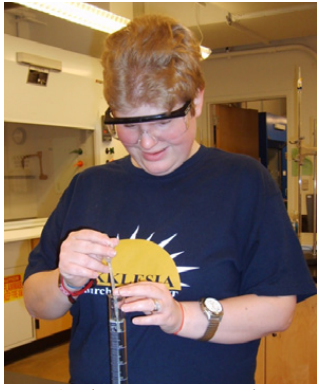
\includegraphics[width=0.9\linewidth]{fig1.png}
    \caption{Volume Determination. The student used the calibrated plastic transfer pipet in the graduated cylinder to measure volumes.}
\end{figure}

Job Access with Speech (JAWS) (Freedom Scientific, Inc., 2010) and Logger Pro 3.6 from Vernier Software and Technology were installed on the computer (Vernier Software \& Technology, 2010) as recommended by Supalo, et al (2007). With these computer applications, different probes and tools, including the Ohaus Scout Pro Balance, were connected to the computer (2007; 2009), which gave the student greater independence. These tools and methods allowed the student to participate in laboratory activities with minimal assistance. 

\subsection*{Lab Familiarization}

Students who are blind have a wide range of spatial awareness, but every student benefits from a well-organized laboratory bench to prevent spills and help with organization (Committee on Chemical Safety, 2003). On the first day, the student with blindness and her assistant walked around the room exploring every section, including the laboratory bench, and locating safety equipment: the exit, fire extinguisher, safety shower, and fume hood. A textured mat was placed on the floor in front of the sink to serve as a “home base,” allowing her to remember the sections of the laboratory. By keeping the laboratory floor free of clutter and obstructions, as suggested by the Committee on Chemical Safety (2003), the student moved independently and self-assuredly. Although laboratory cleanliness is generally considered good practice, it is particularly critical for students who are BLV. 

The computer and any associated probes and balance were always located on the counter to the right of the mat. A Styrofoam block elevated the computer to prevent damage from spills (Rankel \& Winograd, 2010). A food tray placed on the counter between the sink and the computer held any glassware or chemicals used for the day (Committee on Chemical Safety, 2003). Whenever the student needed glassware or chemicals, she could locate the food tray and carefully find the needed item. 

\subsection*{Density}

Students undertake density activities to understand multiple ways to perform calculations and solve problems. The first activity in the revised curriculum for the student with blindness involved finding the densities of a paperweight and a collection of dimes using two different methods of volume determination. Although this activity was not included in the curriculum of the sighted students, it was instructive for the student with blindness to learn to use a balance and measure volumes. The student found the mass of the paperweight using a balance connected to the computer. She then calculated the volume by measuring the height and diameter of the cylindrical paperweight using the millimeter increments on an etched ruler. The assistant had the student feel each etching with her fingernail. Although it was difficult for her to ensure each etching was counted, the student succeeded in measuring the dimensions. This laboratory application solidified her understanding of the metric system. To demonstrate the factor-label method, the professor with blindness used a Perkins Braille writer. 

The student also determined the density of eight dimes using a balance and the graduated cylinder-pipet technique. She found the masses of the empty graduated cylinder, the cylinder filled with water to the 50 milliliter mark (Figures 1), and the eight dimes. She placed the dimes in the cylinder with the 50 mL of water and removed the water above the 50 mL mark with a taped, plastic transfer pipet. She found the mass of the graduated cylinder with the remaining water and dimes. To obtain the mass of the remaining water she subtracted the mass of the cylinder and the mass of the dimes from the mass of the cylinder with the remaining water and dimes. To determine the mass of the displaced water, she subtracted the mass of the remaining water from the mass of the 50 mL of water. By dividing the mass of the displaced water by its density, she was able to determine the volume of the displaced water, and thus the volume of the dimes. 

This activity did not require significant adaptations, and the student could have completed the task independently had she been more familiar with the laboratory techniques. The density determination laboratory allowed her to practice new methods and familiarize herself with the materials and equipment used in the laboratory. These measurements provided the student with an opportunity to manipulate interrelated and quantitative laboratory data. The difference technique employed in this laboratory was paralleled later in the semester in the hydrates laboratory. 

\subsection*{Atomic Spectra: Energy, Light, and the Electron}

Students perform flame emission tests on seven different metal compounds by dipping wire loops into solutions and holding them in the flame of a gas burner. By observing the color in the flame, students must identify the metal cations in unknown solutions (“CHEM 100”, 2010). 

This activity required the student to learn how to light a gas burner. The student with blindness was asked to feel the striker and how the parts moved. Her assistant demonstrated how to hold the striker and create sparks. The assistant positioned the hand of the student and confirmed when the student made sparks (\textit{Figure 2}). As the student listened to the gas run through the burner, the assistant positioned the striker above the burner. Fear and apprehension caused her to jerk the striker away from the burner. If the assistant held the wrist of the student still, she was able to light it! Successfully experiencing the lighting of the burner increased the self-confidence of the student and enabled her to accomplish future tasks. After the student dipped the wire in a solution, the assistant guided the student to the flame by supporting the wrist of the student and described what was happening. The student recorded the results in an Excel™ spreadsheet, which allowed her to analyze the data and complete the experiment. The assistant and the professor with blindness were successful in helping the student learn to light a gas burner. 

\begin{figure}[!h]
    \centering
    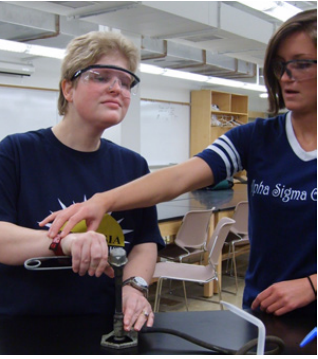
\includegraphics[width=1\linewidth]{fig2.png}
    \caption{Lighting the Gas Burner. This figure illustrates the blind student’s hand placement and the assistance of the sighted assistant as she lit the gas burner.}
\end{figure}

An alternative approach in conducting a flame test involves using an evaporating dish with salts and ethanol. By creating an aluminum foil cylinder shield around the evaporating dish with an opening in the front, a student could detect the resulting flame color using the optical fiber from a spectrometer (L. Rankel, personal communication, March 26, 2010). More spatially aware students with blindness have completed this large-scale flame test with little guidance, thus greatly enhancing their laboratory experience. It is critical for students to practice new skills in the laboratory for them to build confidence before beginning new experiments. If additional time cannot be given, students who are BLV will not feel comfortable with their surroundings, making it difficult to proceed independently with laboratory activities. 

\subsection*{Simulation of Measurement of Hemoglobin in Blood by Spectrophotometry}
This activity requires students to create solutions of known concentrations of iron(III) thiocyanate, use spectrophotometers to create a calibration curve, and determine the concentration of an unknown solution using the calibration curve. The students must make their solutions from the provided stock solutions by using repipeters, droppers, and volumetric flasks. Then they find absorbance values for each solution using a spectrophotometer and record their data in Excel™. With their information and the spectrophotometer, the students determine the concentration of an unknown sample (“CHEM 100”, 2010). 

The student with blindness completed this laboratory almost independently, because she was familiar with the environment. She began by connecting the computer and spectrophotometer and initializing the instrument. Using the pumping and repipetting methods she created all of the solutions necessary for the experiment. Then she filled the volumetric flask with distilled water nearly to the mark using a wash bottle. By pouring the solutions into beakers and by placing them on the food tray in a specific order, the student was able to access the solutions without the help of the assistant. 

The blind student and the assistant counted how many squeezes it took for an eyedropper to fill a cuvette. The student practiced this technique using water to develop a consistent squeezing pattern. After determining the correct number of squeezes, she was able to fill each sample independently. Using Logger Pro and JAWS the student recorded absorbance values in Excel™ for later interpretation. A calibration curve using Braille paper with grid lines and pencil eraser sized adhesive dots can be created using this information (Supalo, 2005). 

\subsection*{Hydrates: An Investigation of Moisture-absorb\-ing Compounds}

Part One of this laboratory activity allows students to qualitatively determine the presence of water in copper(II) sulfate pentahydrate. A test tube containing a sample of hydrated copper(II) sulfate is held over a gas burner. After the water is released from the compound, students try to change the crystals back to their original color and record their observations. In Part Two, they determine the percent of water in hydrated magnesium sulfate by heating the compound in a crucible over a gas burner until the water is evaporated. Students are expected to determine the endpoint by finding a constant mass after completing the heating steps (“CHEM 100”, 2010). 

For Part One, the student with blindness determined the mass of the test tube and the copper (II) sulfate before and after the heating process using a balance, computer, and JAWS. As she heated the test tube, the process seemed endless because the student could not observe the change. It was difficult for her to keep the test tube steady in the flame; therefore, the assistant held her wrist to keep the sample in the flame while maintaining a safe distance. The assistant expedited the process by confirming when the sample was dehydrated, but the student could have completed this independently by finding the mass of the test tube throughout the heating period. After removing the water from the copper (II) sulfate pentahydrate sample, the student used the Color Analysis Laboratory Sensor (CALS) on the outside of the test tube to confirm the change in color. After being calibrated on a piece of white paper, the CALS reports the red, green, and blue components of an object. Thus, the CALS can be used to examine the reaction progress (Mallouk et al, 2010). It was helpful to practice with the CALS using different colors of paper and other materials to help the student understand how the probe worked and how helpful it could be. (The CALS is a prototype device developed at the Pennsylvania State University for the ILAB project and not commercially available from this institution.)

With a different method, the student found the percentage of water in a copper (II) sulfate pentahydrate for Part Two. The student found the mass of a clean and dry crucible, while her assistant prepared the ring stand, wire triangle, and gas burner apparatus to facilitate the process. After heating and cooling the crucible and sample, the student calculated the percentage of water in the hydrated crystal by reweighing it. She confirmed the color change with the CALS. If she had performed Part Two with a sample of magnesium sulfate heptahydrate, as written in “CHEM 100” (2010), she would have been unable to use the CALS because of the absence of color change. 

\subsection*{Chemical Reactions in Everyday Life}

In this activity, students explore solubility rules by mixing different solutions (“CHEM 100”, 2010). They mix nine different solutions together by placing 2-3 drops of each reactant in plastic wells in various combinations. They record whether they observe a reaction, precipitate, cloudiness, or effervescence with each mixture. Then they determine the identity of an unknown solution by testing it with each of their original reactants, with phenolphthalein to determine if it is an acid or base, and with a flame test to determine the cation (“CHEM 100”, 2010). 

The directions were followed as written for a sighted student with minimal modification. The student with blindness directed the assistant to mix 2-3 drops of each reactant in a tray. The student predicted the outcomes based on her understanding of the solubility rules and obtained and recorded observations from the assistant, which was useful for her tests in the lecture portion of the class. The use of the director-assistant method allowed the student to play a more proactive role in conducting the experiment. 

A student who is BLV can perform this laboratory independently by using approximately 5-10 mL of each reactant in a test tube with the aid of a notched syringe or a taped pipet. After letting the reaction occur, the student could confirm her predictions using the “prototypical” Submersible Audible Light Sensor (SALS). The SALS can be used to monitor the progress of a reaction because it provides readings of light levels in real time (Supalo et al, 2008). (The SALS prototype device may become commercially available through the American Printing House for the Blind.)This handheld device can be placed in test tubes and other glassware to detect changes in light during titrations, color changing reactions, and precipitation reactions. The lighter solutions allow more llight to be detected, resulting in a higher pitch; the darker solutions cause a lower pitch (Supalo et al, 2008). Results recorded in Excel™ using JAWS allow the student to notice patterns in reactivity. 

\subsection*{Determination of Citric Acid in Fruit Juices}

The purpose of this laboratory activity intends to determine the concentration of citric acid in orange, grapefruit, lemon, and lime juices by titrating them with a known concentration of sodium hydroxide. Students work with partners to perform titrations on two juices using phenolphthalein as the indicator. They create sample solutions by measuring volumes of the juices and water in graduated cylinders. The students titrate the different juice solutions with sodium hydroxide while constantly swirling the juice sample until one drop of sodium hydroxide causes the permanent appearance of a pink color in the solution (“CHEM 100”, 2010). They perform three trials for each juice. The partners then work with another group to combine their data to determine the concentrations of citric acid in all four juices. 

The student with blindness performed these measurements and titrations independently. She performed the volume measurements using a taped, plastic transfer pipet with a graduated cylinder. Once again, to make it easier to pour the solutions, the student used wash bottles to add the liquids to the graduated cylinders. The arrangement of the supplies was maintained throughout the experience to allow the student to work more independently. The solution was titrated using the SALS and listening for the change in pitch (\textit{Figure 3}). It would have been helpful to practice with the probe more before performing the experiment because the visual endpoint seemed to occur at a different point than the SALS was indicating. This may have resulted from not stirring the solution with the SALS probe, or it may have occurred from lack of practice. This technique could be refined with more time. The student then recorded the volume changes and was able to perform all of the calculations on the computer using Excel™. She performed three trials for two of the assigned juice samples.

\begin{figure}[!htb]
    \centering
    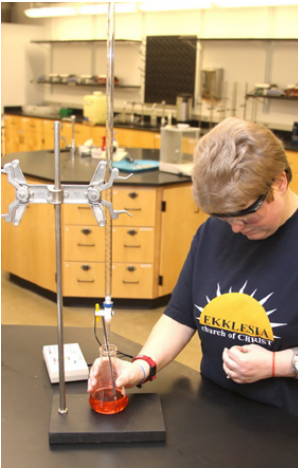
\includegraphics[width=1\linewidth]{fig3.png}
    \caption{Titration with SALS. The figure exhibits the titration equipment and the SALS probe.}
\end{figure}

\section*{CONCLUSIONS}

By taking time to introduce the student with blindness to the laboratory setting, the student became comfortable in her environment. The student worked at her own speed, uninterrupted by impatient classmates. Thus, she was given ample time to contemplate challenging new ideas. Her experience with lighting the gas burner in the beginning of the semester provided an impetus for building confidence and allowed the student to understand how successful she could be with perseverance.  With practice the student became confident in her abilities to find volumes, and she seemed more comfortable with the taped, plastic transfer pipet than the notched syringe. Because the balance was connected to the computer, the readings could be announced by JAWS or later reviewed by the student. These few adapted tools allowed the student to be successful and to work almost self-sufficiently at a variety of experiments.  The student gained confidence in the laboratory, which clearly helped her in the lecture component of the class.  

Students who are BLV must learn modified techniques; therefore they may require more time to accomplish these goals.  Mechanically adept and spatially aware blind students can lead the sighted laboratory partners or participate equally in a regular teaching laboratory situation (Wang, 2007).  Due to time constraints in this case, the assistant often performed the techniques the student had previously mastered, allowing the student to concentrate on key ideas of each activity. 

According to Wild and Allen, “Individual research efforts conducted in isolation—that is, those that are not duplicated or built upon questions raised in the literature—will not move the field forward” (Wild \& Allen, 2009). Some tools and manipulatives are being developed and modified, but more case studies should be performed and documented to obtain data about these tools to prove their reliability. Ultimately, it would be beneficial to compile lists of all known tools, manipulatives, modifications, and case studies into one area and organize it by level and subject.  With more accessible tools, students who are BLV might have greater success in science, which might increase their interest (Supalo et al, 2007).

\section*{ACKNOWLEDGEMENTS}
This work was supported by the National Science Foundation through grant HRD-0435656 and HRD-0726417, and by Truman State University. 

\end{large}
\clearpage
\section*{REFERENCES}\par 

\leftskip 0.25in
\parindent -0.25in 
American Council on Education. (1999). \textit{College freshmen with disabilities: A biennial statistical profile}. Washington, DC: Henderson, C. 

Americans with Disabilities Act 1990. Pub. Law 101-336. (1990). Retrieved from: \url{http://thomas.loc.gov/cgibin/bdquery/z?d101:SN00933:@@@L|TOM:/bss/d101query.html}.  

Cetera, M. (1983). Laboratory Adaptations for Visually Impaired Students: Thirty Years in Review. \textit{Journal of College Science Teaching, 12} (5), 384-393. 

“CHEM 100”. (2010). Truman State University. Retrieved from:
\url{http://chemlab.truman.edu/CHEM100.htm}. 

Committee on Chemical Safety. (2003). \textit{Safety in academic chemistry laboratories: Accident prevention for college and university students: Vol. 1} (7th ed.). Washington, D.C.: American Chemical Society. 

De Lucchi, L. and Malone, L. (1982). Chapter 10: Science activities for the visually impaired. In \textit{S. Mangold (Ed.), A teacher’s guide to the special educational needs of blind and visually handicapped children} (pp. 72-93). New York, New York: American Foundation for the Blind. 

Erwin, E., Perkins, T., Ayala, J., Fine, M., \& Rubin, E. (2001). You don’t have to be sighted to be a scientist, do you?. \textit{Journal of Visual Impairment and Blindness, 95} (6), 338-352. 

Freedom Scientific, Inc. (2010). JAWS for windows screen reading software [software]. St. Petersburg, Florida: \$1095. 

Individuals with Disabilities Education Act of 1975. Pub. Law No. 94-142. (1975). Retrieved from: \url{http://www.ada.gov/cguide.htm#anchor65310}.

Individuals with Disabilities Education Improvement Act of 2004. Pub. Law No. 108- 446.(2004). Retrieved from: \url{http://idea.ed.gov/download/statute.html}. 

Mallouk, T., Supalo, C., Hill, A., Kreuter, R., Carlsen, B., Roth, A.,…Bodner, G. (2010). Independent Laboratory Access for the Blind. Retrieved from: \url{http://ilab.psu.edu/index.html}. 

Miner, D., Nieman, R., Swanson, A., and Woods, M. (Ed.) (2001). \textit{Teaching Chemistry to Students with Disabilities: A Manual for High Schools, Colleges, and Graduate Programs} (4th ed.). Washington, DC: The American Chemical Society.

Rankel, L. \& Winograd, M. (2010). Getting in on science: Strategies for teaching chemistry,physics, and physical science with labs for blind and visually impaired students. \textit{AER Report, 27} (1). 

Rehabilitation Act of 1973. Pub. Law No. 93-112. (1973). Retrieved from: \url{http://www.dotcr.ost.dot.gov/documents/ycr/REHABACT.HTM}. 

Schmeidler, E. \& Kirchner, C. (2007). Adding Audio Description: Does it make a Difference? \textit{Journal of Visual Impairment and Blindness, 95} (4), 197-212. 

Supalo, C. (2005). Techniques to Enhance Instructors' Teaching Effectiveness with Chemistry Students Who Are Blind or Visually Impaired. \textit{Journal of Chemical Education, 82} (10), 1513-1518. 

Supalo, C., Mallouk, T., Amorosi, C., Rankel, L., Wohlers, H., Roth, A. \& Greenberg, A. (2007). Talking Tools to Assist Students Who are Blind in Laboratory Courses. \textit{Journal of Science Education for Students with Disabilities, 12} (1), 27-32. 

Supalo, C., Mallouk, T., Rankel, L., Amorosi, C., and Graybill, C. (2008). Low-Cost Laboratory Adaptations for Precollege Students Who Are Blind or Visually Impaired. \textit{Journal of Chemical Education, 85} (2), 243-247. 

Supalo, C., Mallouk, T., Amorosi, C., Lanouette, J., Wohlers, H.D., and McEnnis, K. (2009). Using Adaptive Tools and Techniques To Teach a Class of Students Who Are Blind or Low- Vision. \textit{Journal of Chemical Education, 86} (5), 587-590. 

Vernier Software \& Technology Company. (2010). Logger Pro [software]. Retrieved from: \url{http://www.vernier.com/}. 

Wang, L. (2007). \textit{Chemical and Engineering News}, 85, No. 30, 36-40, retrieved from: \url{http://pubs.acs.org/cen/education/85/8530education1.html} (accessed August 2011).

Wexler, A. (1961). \textit{Experimental science for the blind: An instructional manual}. London: Pergamum Press, Inc. 

Wild, T. \& Allen, A. (2009). Policy analysis of science-based best practices for students with visual impairments. \textit{Journal of Visual Impairment and Blindness, 103} (2), 113-117. 

Willoughby, D. M., Duffy, S. L. M. (1989). \textit{Handbook for Itinerant and Resource Teachers of Blind and Visually Impaired Students}. Baltimore: National Federation of the Blind. 

Wohlers, H.D. \& Hoffmann, J. (2008). Using talking and audible laboratory tools in the Chemistry 100 Course-Chemistry for Contemporary Living. Institutional Review Board:Truman State University.

\end{document}